\begin{frame}{Problem}
	\centering
	\Large
	Given a terrain and some observers, we want to calculate a path that has the least chance of detection

	\note{
		Now that that's in place, let's back up and figure out why we would want this
	}
\end{frame}

\subsection{Motivation}
\begin{frame}{Military}
	Planning troop movements in enemy territory

	\vspace{0.5cm}
	\centering
	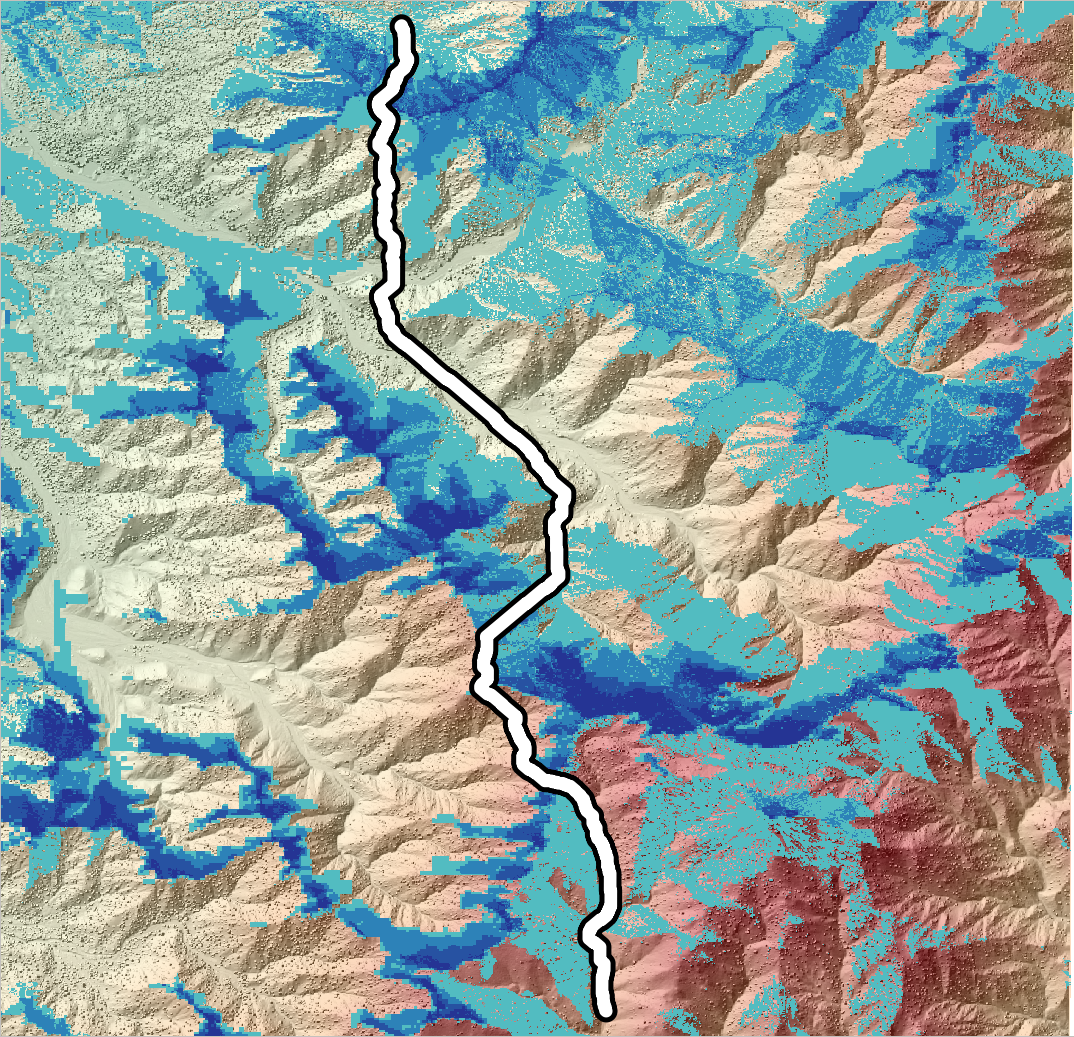
\includegraphics[width=0.35\textwidth]{motivation-military}
\end{frame}

\begin{frame}{City planning}
	Visually unappealing structures

	\vspace{0.5cm}
	\centering
	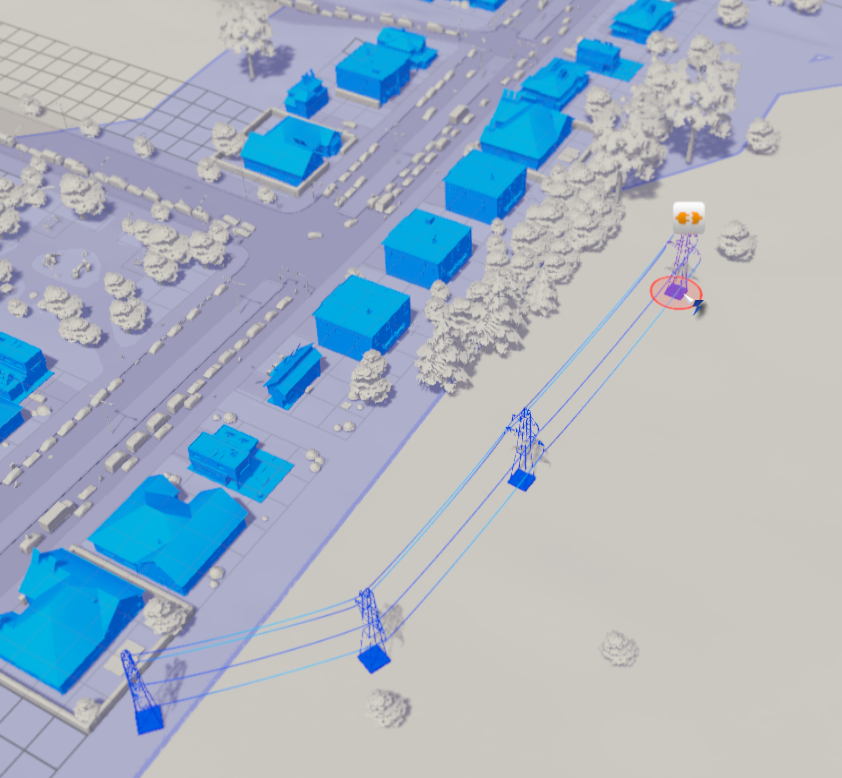
\includegraphics[width=0.35\textwidth]{motivation-city}
\end{frame}

\begin{frame}{Virtual environments}
	Video games

	\vspace{0.5cm}
	\centering
	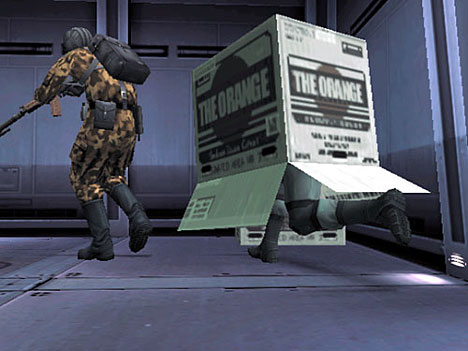
\includegraphics[width=0.45\textwidth]{motivation-virtual}
\end{frame}


\subsection{Terrain}
\begin{frame}{What's a terrain?}
	\begin{itemize}
		\item A map
		\item Elevation
	\end{itemize}

	\note{
		For the rest of the lecture, we'll assume that a terrain is a grid plus a defined height function.
		Note that this representation of terrains can't handle non-convex shapes, so we can't model tunnels or caves using this definition.
	}
\end{frame}

\begin{frame}{Digital Elevation Model}
	\centering
	\only<1>{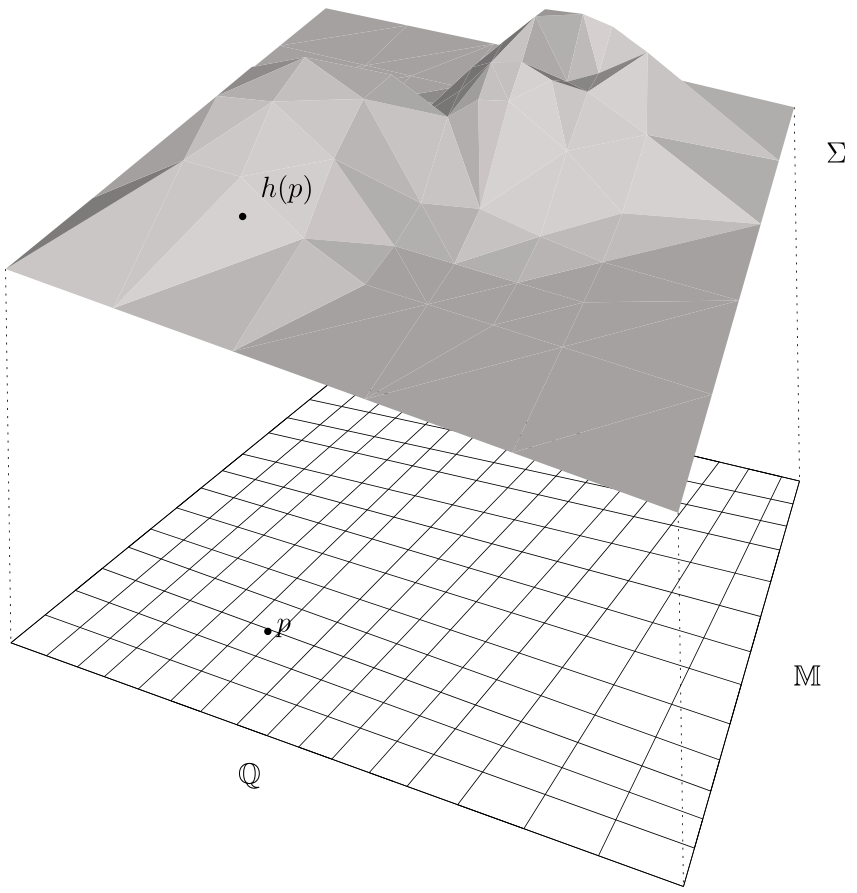
\includegraphics[width=0.6\textwidth]{DEM}}
	\only<2>{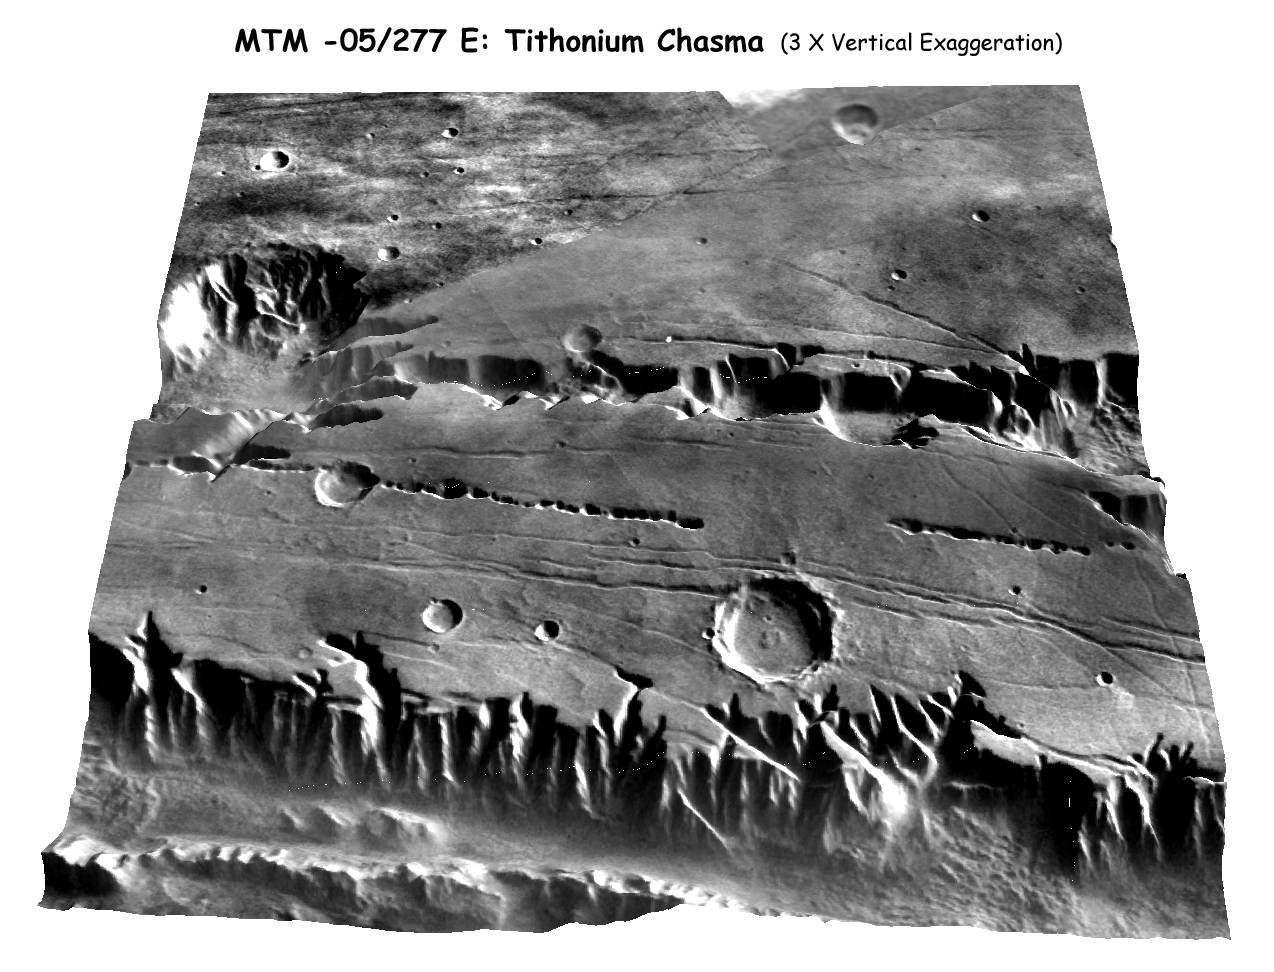
\includegraphics[width=0.8\textwidth]{DEM-mars}}

	\note{
		In particular, we'll be working with DEMs, since they are a common format
	}
\end{frame}

\begin{frame}{Example}
	\centering
	\only<1>{
\includegraphics[width=\examplewidth]{empty}}
	\only<2>{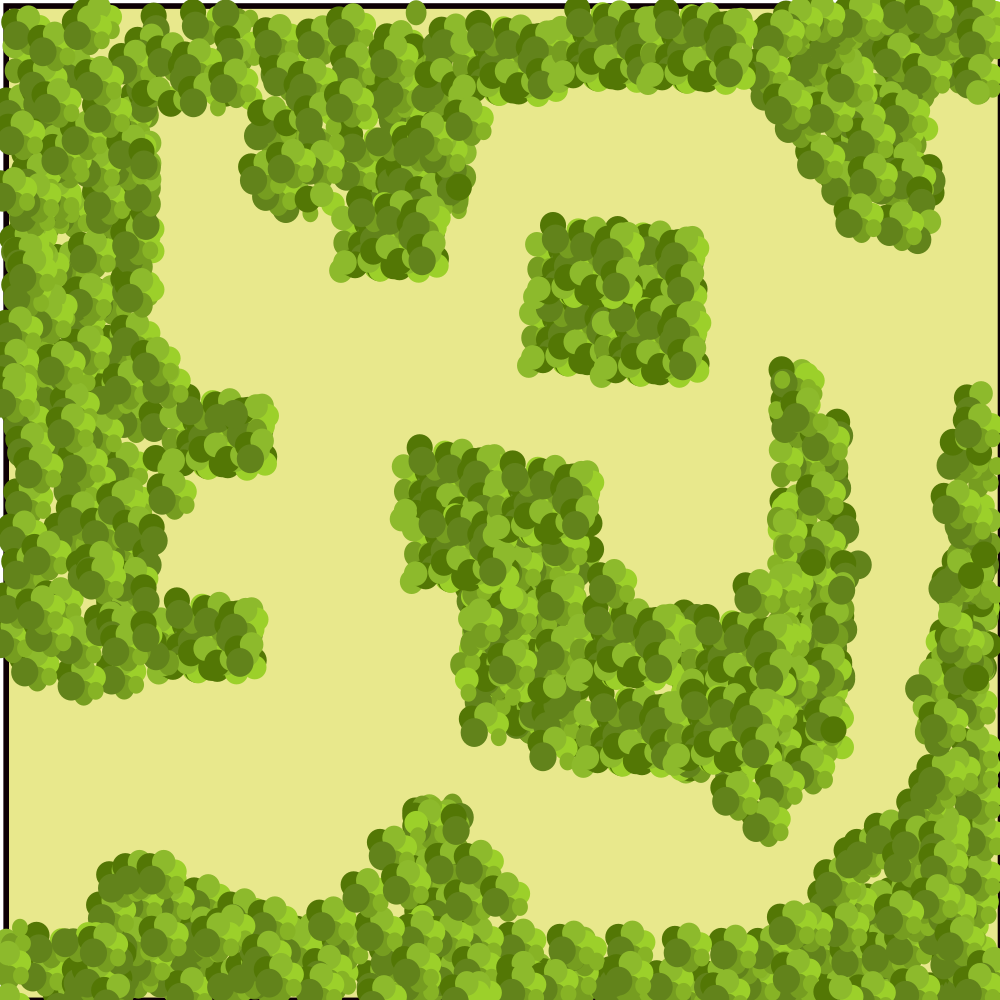
\includegraphics[width=\examplewidth]{terrain}}

	\note{
		Throughout this lecture, we'll work with a very simple example terrain to make it clear what the algorithm is doing.
		We'll start with our grid.

		For elevation, we introduce some trees.
		We do this simply because 3D terrains are hard to get across on slides.
	}
\end{frame}


\subsection{Observers}
\begin{frame}{Observer}
	\begin{itemize}
		\item Entity on the terrain
		\item Visible grid points \note{Those with a clear line of sight}
	\end{itemize}
\end{frame}

\begin{frame}{In our example}
	\centering
	\only<1>{
		\exampleimg{observers}
		\note{So say these dots on the terrain are our observers. We're just going to assume that these are given}
	}%
	\only<2>{
		\exampleimg{observers_visibility}
		\note{
			The next step is to figure out, for each observer, which points on the terrain are visibile and which aren't.
			Of course, the definition of visibilty can be whatever you want it.
			Here, and in the paper we're about to get to, we use that a line from the observer to the point cannot intersect with the height function.
		}
	}%
	\only<3>{
		\exampleimg{observers_line_of_sight}
		\note{However, this isn't realistic as visibily degenerates with distance}
	}%
	\only<4>{
		\exampleimg{observers_line_of_sight_one}
		\note{So we determine, for each observer, how well they can see each point}
	}%
	\only<5>{
		\exampleimg{observers_line_of_sight_all}
		\note{
			And when aggregate that (if we sum the visibility increase from 11 to 12 observers seeing a point would be the same as 1 to 2, so that's not good),
			we end up with the visibility map
		}
	}
\end{frame}


\subsection{Paths}
\begin{frame}{Goal}
	\centering\Large
	Getting from A to B with the lowest chance of detection
	\note{Let's go back to what we actually wanted to achieve here}
\end{frame}

\begin{frame}{Example}
	\centering
	\only<1>{\exampleimg{observers_line_of_sight_all}}%
	\only<2>{\exampleimg{observers_line_of_sight_all_points}}%
	\only<3>{\exampleimg{observers_line_of_sight_all_path}}
\end{frame}


